\documentclass[10pt]{article}
\usepackage[margin=0.85in]{geometry}
\usepackage{graphicx}
\usepackage{booktabs}
\usepackage{amsmath}
\usepackage{array}
\usepackage{microtype}
\usepackage{hyperref}
\usepackage{xcolor}
\usepackage{enumitem}
\usepackage{authblk}
\usepackage{siunitx}
\usepackage{caption}
\usepackage{subcaption}
\usepackage{float}
\hypersetup{colorlinks=true,linkcolor=blue,citecolor=blue,urlcolor=blue}
\setlist[itemize]{leftmargin=*,nosep}
\newcommand{\sepr}{\mathrm{SEPR}}
\newcommand{\pp}{\,\mathrm{pp}}

\title{From Evidence to Intervention: State Error Propagation and Abstention in Longitudinal LLM-Mediated Psychological Support}
\author{Naimur Rahman}
\affil{Independent Researcher, London, United Kingdom\\ORCID: 0009-0004-2794-077X}
\date{September 2026}

\begin{document}
\maketitle

\begin{abstract}
Longitudinal LLM-mediated support depends not only on generating plausible responses but on maintaining the right user state across repeated interactions. We study how errors in a persistent representation of situation, appraisal, emotion, regulatory goal, and prior exercise propagate into downstream intervention decisions. A controlled synthetic benchmark compares three architectures using Qwen3-8B: dialogue history only (A), naive structured state (B), and reliability-aware structured state with provenance, temporal scope, contradiction handling, and deferral (C). Six evidence conditions are evaluated over five observations per trajectory. A pre-analysis computational amendment fixed a 20-base held-out pilot before held-out performance was inspected, yielding 1,590 primary and 600 matched-control turn outcomes. Structured state did not improve clean-condition state recall over history prompting (B$-$A $=-8.83$ percentage points (pp), 95\% bootstrap CI $[-19.83,0.50]$). Injected unsupported inference increased persistence in B by $28.33\pp$ $[16.67,41.67]$, but the associated decision-error increase was not clearly separated from zero. Most importantly, C reduced absolute propagation burden relative to B ($-18.11\pp$ $[-26.48,-10.60]$) while sharply reducing coverage ($-76.98\pp$ $[-89.20,-63.33]$) and increasing conditional state-error propagation rate (SEPR) by $10.18\pp$ $[5.27,15.41]$. The reference-mode sensitivity analysis showed the same direction. These results show that lower absolute error burden can be obtained through selectivity without better conditional state reliability. Reliability claims for longitudinal LLM systems should therefore report state-error incidence, conditional propagation, propagation burden, and coverage jointly rather than treating abstention-driven reductions as sufficient evidence of improved reliability.
\end{abstract}

\section{Introduction}
Long-term memory is becoming a standard component of LLM assistants and agents. Existing work has shown that persistent memory can improve retrieval and personalization \cite{zhong2024memorybank,wu2024longmemeval}, while newer benchmarks increasingly test temporal updates and memory structure rather than isolated fact recall \cite{shutova2026structmemeval}. In psychologically oriented interaction, however, persistent state creates an additional reliability problem: a system can remember the wrong appraisal, retain an inference that was never stated, or continue acting on a state the user has explicitly superseded.

This distinction matters because psychologically meaningful support is not reducible to fluent wording. Emotional validation concerns whether an emotion is understandable in context, whereas cognitive reappraisal concerns changing construals without simply inventing a more positive story \cite{gross1998emotion,kuo2022validation,uusberg2023expanded}. Recent computational work has begun to model appraisals and cognitive reframing \cite{agarwal2025appraisals,ruder2025appraisal}, and multi-turn mental-health and emotional-support benchmarks evaluate increasingly sophisticated dialogue behavior \cite{wang2024patientpsi,zhao2024esceval}. Yet a narrower systems question remains underexplored: when an intermediate psychological state is wrong, does that error survive into later observations and change the intervention decision?

We study this as an evidence-state reliability problem. The experiment separates three questions that are often collapsed: whether the system's active state is correct; whether an erroneous active state causally changes a typed intervention decision under controlled repair/replay; and whether a system proceeds at all. This is motivated by the broader observation that intermediate-state failures can be hidden by apparently valid downstream outputs \cite{rahman2026esr}.

Our main finding is adverse to the original reliability-aware hypothesis. The reliability-aware architecture reduces the number of turns carrying attributed propagation, but it does so together with a large coverage collapse, while its conditional propagation rate among surviving erroneous-state exposures is higher. This yields a practical lesson: \emph{abstention can lower absolute error burden without establishing better conditional state reliability}.

\paragraph{Contributions.} We provide:
\begin{itemize}
  \item a controlled longitudinal benchmark with synthetic non-clinical scenarios, six evidence degradations, five scheduled observations, and matched fault-free controls;
  \item a typed state-error propagation estimand (SEPR) using single-slot repair/replay attribution rather than response-level plausibility alone;
  \item a three-architecture comparison that separates state accuracy, conditional propagation, absolute propagation burden, and coverage;
  \item a negative-result analysis showing that naive structured memory does not automatically improve clean retention, and that reliability-aware gating can trade coverage for lower burden while worsening conditional propagation;
  \item an executable, source-frozen reproducibility package with deterministic benchmark generation, held-out guards, paired bootstrap analysis, and explicit post-design amendments.
\end{itemize}

\section{Related Work}
\subsection{Psychological state and intervention structure}
Appraisal theories distinguish situations, interpretations, emotional responses, and regulation processes \cite{gross1998emotion}. Reappraisal changes the construal of an event rather than merely producing positive language \cite{uusberg2023expanded}; validation, likewise, concerns acknowledging the intelligibility of an emotional response in context rather than endorsing an unverified external claim \cite{kuo2022validation}. Computational work has examined relations between cognitive distortions and appraisals \cite{agarwal2025appraisals} and the reliability of LLM-based appraisal annotation \cite{ruder2025appraisal}. Our benchmark uses these distinctions only as a constrained ontology for synthetic, non-clinical support; it does not claim clinical validity.

\subsection{Longitudinal memory}
MemoryBank and related systems demonstrate the utility of persistent memory in sustained interaction \cite{zhong2024memorybank}. LongMemEval evaluates extraction, multi-session and temporal reasoning, knowledge updates, and abstention over controlled histories \cite{wu2024longmemeval}; newer work examines the organization of memory structures themselves \cite{shutova2026structmemeval}. In mental-health data, CliniCIRCA reconstructs temporally grounded patient journeys from unstructured clinical narratives, illustrating the importance of temporal recovery when evidence is distributed across a longitudinal record \cite{zhang2026clinicirca}. Our focus is narrower and non-clinical: not whether memory improves downstream task accuracy or clinical timeline reconstruction in general, but how a known error in an active psychological-state slot propagates to a later intervention decision.

\subsection{Evaluation reliability and selective prediction}
LLM-as-a-judge methods are convenient but can exhibit systematic bias and disagreement with humans \cite{zheng2023judge,chen2024judges}. We therefore separate deterministic decision-level endpoints from semantic response-text evaluation. The final experiment used a manual-audit-only evaluator mode after no automated evaluator was validated prospectively. More generally, selective prediction frames abstention as a risk--coverage trade-off \cite{geifman2019selectivenet}. Our results show why that trade-off must be made explicit in longitudinal state systems: lower absolute error burden at very low coverage is not equivalent to lower conditional propagation given an error exposure.

\section{Research Questions and Prospective Criteria}
The source package defined four research questions before model execution. The protocol was source-hashed and frozen internally but was not externally registered as a preregistration.

\begin{description}[leftmargin=0.5cm,style=nextline]
\item[RQ1/H1.] Does structured state improve clean representation/retention relative to dialogue-history prompting? H1 required the paired 95\% CI for clean B$-$A state recall to lie above zero, without an undermining precision trade-off.
\item[RQ2/H2.] Can an incorrect structured state persist and affect downstream intervention decisions? H2 required increased post-injection persistence and downstream decision-error burden relative to matched no-fault controls, with directionally consistent trajectory-cluster intervals.
\item[RQ3/H3.] Does reliability-aware state management reduce error propagation relative to naive structured state? H3 required C$-$B SEPR $\leq -0.05$ with a 95\% interval below zero. Coverage loss greater than 10 percentage points was prospectively defined as a material trade-off.
\item[RQ4/H4.] Can automated evaluation reliably detect state-induced semantic failures? This arm was not tested because no automated evaluator passed the prospective validation path; semantic fidelity therefore remained unvalidated in the confirmatory analysis.
\end{description}

\section{Methods}
\subsection{Synthetic longitudinal benchmark}
The V2 benchmark contains 12 authored everyday scenario families and eight longitudinal transition archetypes. Scenarios concern non-clinical adult social-evaluative situations and exclude crisis, self-harm, diagnosis, medication, abuse, and clinical relationships. Each base trajectory contains five observations at days 0, 3, 7, 10, and 14. The latent specification is created before dialogue rendering, and later user turns are exogenous: generated assistant responses are not fed back into subsequent user evidence. This preserves paired evidence across architectures but prevents inference about how a real person would react to the intervention.

The active psychological state is typed into situation, appraisal, emotion, regulatory goal, and prior exercise and feedback fields. The intervention family is constrained to emotional validation, cognitive reappraisal, or clarify/defer. Six conditions are applied prospectively where applicable: clean, missing evidence, contradictory evidence, superseded appraisal, unsupported inference, and stale state. Unsupported-inference and stale-state conditions additionally have matched fault-free controls. Applicability is determined from the latent trajectory shape before model execution: only cells classified prospectively as clean or stratified enter the primary matrix. Contradictory evidence is excluded when a natural retraction would confound the injected contradiction or when the perturbation-turn appraisal cannot support the intended contrast; superseded appraisal is excluded when the natural trajectory already contains the same correction or the perturbation-turn appraisal makes the intended retraction inapplicable. These rules yield 13 of 20 applicable pilot bases for each of those two conditions, versus 20 of 20 for the other four.

\subsection{Architectures}
\textbf{A (History)} receives the full available user-evidence prefix at each observation and has no persistent state object. It emits transient typed targets with its intervention decision for evaluation.

\textbf{B (Structured)} uses a shared extractor to propose state updates from the latest evidence and applies a last-write persistence rule. It has no reliability annotations in its decision-time state view.

\textbf{C (Reliability-aware)} receives the same user evidence and the same extraction proposals as B, but maintains provenance, source turn, temporal scope, explicit/inferred status, contradiction and supersession handling, and a clarification/defer mechanism. C never receives latent truth or future turns. Thus the primary B--C contrast changes state-management logic rather than evidence or the extraction model.

\subsection{Model and inference}
All architectures use \texttt{Qwen/Qwen3-8B}, Hugging Face revision \texttt{b968826d9c46dd6066d109eabc6255188de91218}, served with vLLM 0.29.0 in BF16. The recorded runtime used Transformers 5.17.0, PyTorch 2.13.0+cu130 and CUDA 13.0; the serving fingerprint was \texttt{vllm-0.29.0-33dd102b}. Non-thinking mode is enforced with \texttt{enable\_thinking=false}. Generation uses temperature 0.7, top-$p$ 0.8, top-$k$ 20, min-$p$ 0, maximum 1,800 tokens, and inference seed 263901. Model-file hashes and the serving fingerprint are stored in the provenance package.

\subsection{Pilot amendment and execution}
The original held-out design contained 100 base trajectories. After HLD-001--005 had been executed, but before any held-out scientific performance was inspected, a computational-feasibility amendment fixed a 20-base application/preprint pilot. The amendment retained HLD-001--005 and selected 15 further bases by deterministic SHA-256 ranking of the remaining IDs, independent of content or outcomes. The final sample contained 20 clean, 20 missing-evidence, 13 contradictory-evidence, 13 superseded-appraisal, 20 unsupported-inference, and 20 stale-state primary variants: 106 primary variants $\times$ 3 architectures $\times$ 5 observations = 1,590 primary outcomes, plus 600 matched-control outcomes, for 2,190 total turn outcomes.

A second execution-only amendment was made before the 15 additional bases were run. A calibration-only smoke test showed that running five independent base trajectories concurrently reduced wall time while preserving model identity, parser validity, and non-thinking mode. Within each base, the frozen call order remained sequential. The first five held-out bases were therefore executed serially and the remaining 15 in three five-base waves. Because stochastic generation can differ under batching even with fixed seeds, this execution heterogeneity is retained as a limitation rather than treated as bitwise equivalence.

\subsection{Metrics}
State recall and precision compare the evaluated typed state against the synthetic latent specification. Decision error is a deterministic typed mismatch in the selected intervention target or family; it is distinct from semantic response-text fidelity.

For B and C, the primary propagation endpoint is the \emph{state-error propagation rate} (SEPR). An exposure is an erroneous active state-slot immediately before a downstream decision. For each exposure, the pipeline replays the original decision and performs a single-slot repair using evaluator-only reference information. An exposure is attributed as propagated when repairing that slot changes the erroneous decision in the expected direction while the replay reproduces the decision. Failed/non-reproducing cases are kept as ambiguous. Formally,
\[
\sepr = \frac{\text{repair-attributable propagating error exposures}}{\text{erroneous active state-slot exposures}}.
\]
SEPR is undefined at zero exposures and is not estimated for A because A has no persistent state intervention point. Since B and C can change which errors survive into the denominator, we also report state-error exposure counts, propagation burden (eligible turns containing any attributed propagated error), and decision coverage. Decision coverage is the fraction of eligible turns on which the architecture proceeds rather than defers. We additionally report \emph{decision-reliable coverage}, the fraction of eligible turns on which the architecture both proceeds and has no deterministic typed decision error:
\[
\text{decision-reliable coverage}=\frac{\#(\text{proceeded turns with no typed decision error})}{\#(\text{eligible turns})}.
\]
This metric is independent of semantic response-text fidelity; the latter was not available as a validated automated endpoint. This distinction is central: a system can reduce propagation burden by preventing exposures or abstaining while still having a high conditional SEPR among surviving exposures.

All confirmatory intervals use 2,000 paired bootstrap repetitions clustered by base trajectory (seed 77129). Turns are not treated as independent participants.

\section{Results}
\subsection{Overall behavior}
Across the 1,590 primary outcomes, A had state recall 0.6412, state precision 0.6817, decision-error rate 0.7396, and coverage 1.0000. B had recall 0.5194, precision 0.6570, decision-error rate 0.8585, and coverage 0.9943. C had recall 0.4789, precision 0.7320, decision-error rate 0.8358, but coverage only 0.2245. B produced 795 erroneous state-slot exposures, of which 595 were attributed as propagated (SEPR 0.7484); C produced 514 exposures, 437 propagated (SEPR 0.8502).

\begin{table}[t]
\centering
\caption{Overall primary descriptives. SEPR is defined only for persistent-state architectures B and C.}
\label{tab:overall}
\begin{tabular}{lrrrrrr}
\toprule
Arch. & Recall & Precision & Decision error & Coverage & Exposures & SEPR \\
\midrule
A & 0.641 & 0.682 & 0.740 & 1.000 & -- & -- \\
B & 0.519 & 0.657 & 0.859 & 0.994 & 795 & 0.748 \\
C & 0.479 & 0.732 & 0.836 & 0.225 & 514 & 0.850 \\
\bottomrule
\end{tabular}
\end{table}

\subsection{H1: structured state did not improve clean recall}
On the clean condition, B$-$A state recall was $-0.0883$ (95\% CI $[-0.1983,0.0050]$), so the prospective H1 criterion was not met. The precision difference was small and uncertain ($-0.0039$, $[-0.0791,0.0616]$). In this short-history benchmark, explicitly persisting a structured state did not improve representation retention relative to providing the full evidence prefix.

\subsection{H2: injected unsupported inference persisted, but a cascade was not established}
For unsupported inference, B's fault-minus-control persistence increased by $0.2833$ (95\% CI $[0.1667,0.4167]$). The corresponding decision-error difference was $0.0200$ with an interval touching zero ($[0.0000,0.0600]$). For stale state, persistence increased by $0.1000$ ($[0.0000,0.2500]$), while the decision-error difference was exactly 0 in this pilot. Thus an unsupported inference clearly persisted in the structured state, but the stronger prospective claim that persistence produced a downstream decision-error cascade was not established.

\subsection{H3: lower absolute burden accompanied worse conditional propagation and severe coverage loss}
The primary C$-$B SEPR difference was $+0.1018$ (95\% CI $[0.0527,0.1541]$), the opposite of the prospectively required improvement. At the same time, C reduced propagation burden by $-0.1811$ ($[-0.2648,-0.1060]$) and coverage by $-0.7698$ ($[-0.8920,-0.6333]$). Decision-reliable coverage also fell by $-0.0981$ ($[-0.1473,-0.0537]$). Figure~\ref{fig:effects} makes the trade-off explicit.

\begin{figure}[t]
\centering
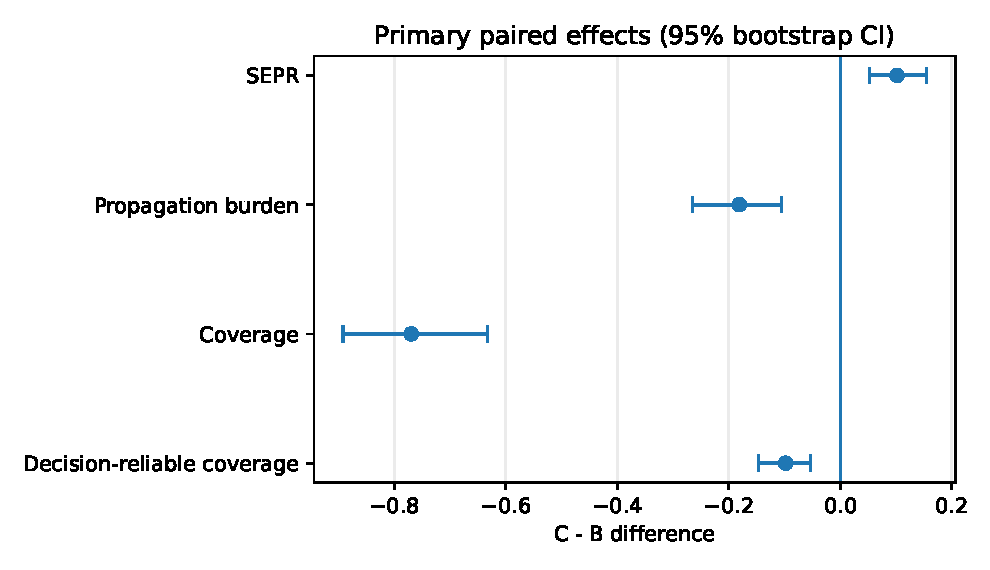
\includegraphics[width=0.95\linewidth]{figures/primary_effects.pdf}
\caption{Primary paired C$-$B effects with 95\% trajectory-cluster bootstrap intervals. Negative propagation burden indicates fewer eligible turns with attributed propagation; positive SEPR indicates a higher conditional propagation rate among surviving erroneous-state exposures.}
\label{fig:effects}
\end{figure}

The pre-specified reference-mode sensitivity analysis preserved the primary directions. C$-$B was $+0.1075$ ($[0.0547,0.1648]$) for SEPR and $-0.2000$ ($[-0.2784,-0.1266]$) for propagation burden. Coverage was $-0.7468$ ($[-0.8785,-0.6050]$), and decision-reliable coverage was $-0.0911$ ($[-0.1418,-0.0474]$). All four intervals excluded zero in the same direction as the primary contrasts, so the result was not mode-dependent under the protocol's sensitivity rule.

Post-freeze, analysis-only robustness checks were also directionally consistent and did not redefine the prospective H3 criterion. For the primary H3 contrast, a 10,000-draw paired base-cluster bootstrap gave a C$-$B SEPR interval of $[0.0539,0.1544]$, while clustering instead by context family gave $[0.0421,0.1608]$. All 20 leave-one-base-out SEPR estimates remained positive (range $+0.0894$ to $+0.1126$). Propagation-burden and coverage differences remained negative under the 10,000-draw bootstrap, context-family clustering, and all 20 leave-one-base-out analyses; repeating the 2,000-draw bootstrap across five fixed seeds did not change these directions. These are secondary stability diagnostics of the frozen pilot, not cross-model, external, or clinical robustness.

\subsection{Condition-level decomposition}
C's coverage was lower than B in every condition, ranging from 0.140 under stale state to 0.330 on clean trajectories, compared with 0.980--1.000 for B (Figure~\ref{fig:coverage}). C's SEPR was numerically higher in all six conditions. The clearest condition-level increase occurred under superseded appraisal: $+0.1383$ (95\% CI $[0.0576,0.2389]$). Conversely, the largest reduction in propagation burden occurred under stale state ($-0.3900$, $[-0.5100,-0.2598]$), paired with an $-0.8600$ coverage difference. The mechanism is therefore not a simple ``C is worse'' result: C filtered or deferred many opportunities for propagation, but among erroneous state exposures that remained active, the conditional propagation probability did not improve.

\begin{figure}[t]
\centering
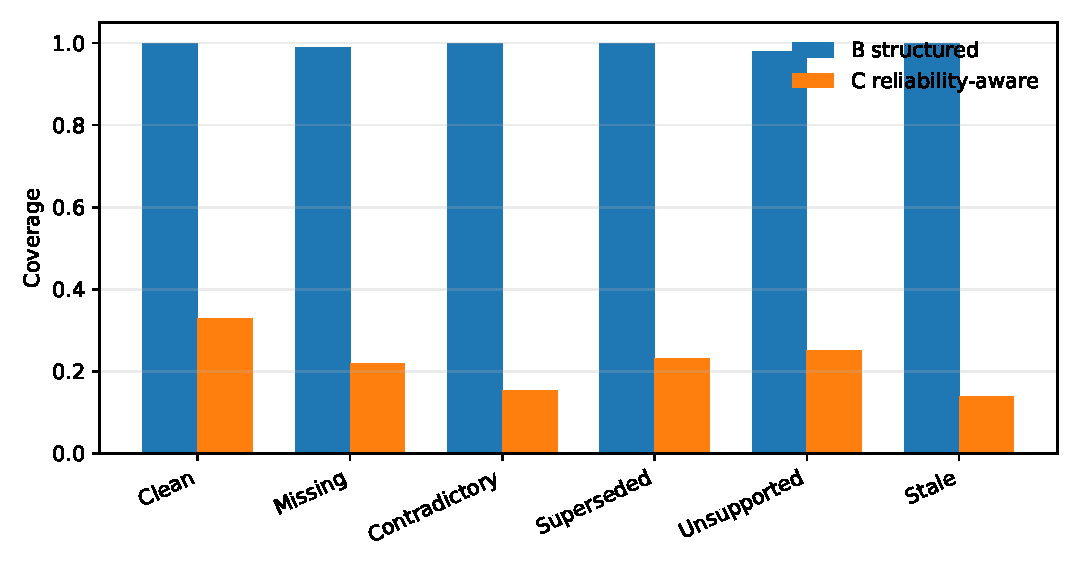
\includegraphics[width=0.95\linewidth]{figures/coverage_by_condition.pdf}
\caption{Decision coverage by condition. Reliability-aware C proceeded far less often than naive structured B in every degradation condition.}
\label{fig:coverage}
\end{figure}

\begin{figure}[t]
\centering
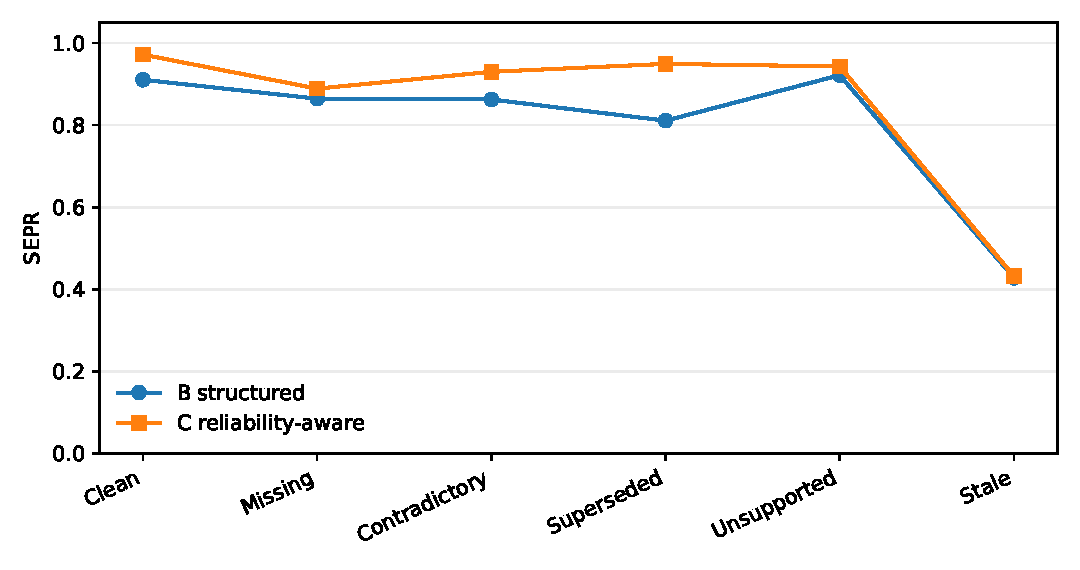
\includegraphics[width=0.95\linewidth]{figures/sepr_by_condition.pdf}
\caption{Condition-level SEPR for B and C. Conditional propagation was not lower for C in any condition; superseded appraisal showed a clear adverse C$-$B difference.}
\label{fig:seprcond}
\end{figure}

\subsection{Semantic response-text audit}
The final evaluator mode was \texttt{manual\_audit\_only}; no automated semantic-fidelity model was validated for confirmatory use, so H4's automated-detection arm is not tested. The private deblinding key records \texttt{automated\_failure} as null for all 324 sampled items; sensitivity, specificity, agreement, and Cohen's $\kappa$ against an automated semantic evaluator are therefore undefined rather than zero.

A deterministic seed selected 10 pilot bases for a blinded packet of 324 response-text items. One non-clinical author rater completed all items while blinded to architecture and condition. The final overall judgments were 322 pass, one fail, and one genuinely ambiguous item (323 evaluable; descriptive failure proportion $1/323=0.0031$). The initial rating interface defaulted the overall field to ``ambiguous''; before deblinded aggregate reporting, this UI artifact was corrected through explicit author confirmation, and the remaining ambiguous items were reviewed with no default selection. The correction history is retained in the reproducibility notes. Optional interface subfields are not used for manuscript inference.

This audit is reported only as descriptive author-blinded evidence because the rater was also the study author/developer and had seen aggregate experiment results before audit completion. It is not independent clinical validation. These response-text judgments are also a different construct from the deterministic typed decision-error metric and are not used to invalidate or replace decision-level outcomes.

\section{Discussion}
\subsection{Structured memory is not automatically reliable memory}
The clean-condition result cautions against equating persistence with retention quality. B had access to an explicit structured state, yet did not improve state recall relative to full-history prompting. The benchmark histories are deliberately short, so this does not imply that structured memory is useless in long contexts; rather, it shows that state structure itself is not sufficient evidence of longitudinal reliability.

\subsection{The abstention trap}
The central result is the divergence between absolute and conditional reliability. C produced fewer erroneous-state exposures and fewer turns with attributed propagation, but proceeded on only 22.45\% of primary turns and had a higher SEPR among the errors that remained active. A system designer reporting only absolute error counts could therefore describe C as safer, while a designer reporting only conditional SEPR could describe it as worse. Both descriptions omit a necessary part of the risk--coverage picture.

For reliability-aware agents, we therefore recommend a four-part report: (1) state-error incidence/exposures, (2) conditional propagation given an exposure, (3) absolute propagation burden per eligible turn, and (4) coverage or abstention. Reliability improvements should not be claimed from one quantity alone.

C's overall state precision (0.7320) was higher than B's despite lower state recall and much lower decision coverage. This is not contradictory: state precision is computed over asserted state slots, excluding values represented as unknown or hypothesis, so a more selective state representation can increase precision while withholding uncertain assertions and reducing recall or downstream coverage. The pilot does not identify this as the sole causal mechanism, and the precision increase should not be interpreted as better end-to-end reliability.

\subsection{Unsupported inference is sticky even when its downstream effect is small}
The H2 decomposition separates persistence from consequence. Unsupported inference persisted strongly under B, but the pilot did not establish a corresponding decision-error increase with a confidence interval separated from zero. This is useful mechanistically: a memory system can be wrong for multiple turns without every wrong state changing the chosen intervention. Future work should model the transition from state error to decision sensitivity explicitly rather than assuming persistence implies downstream harm.

\section{Limitations}
This is a small, synthetic, non-clinical pilot and should be interpreted accordingly. First, the benchmark uses authored latent truth, templated language, five observations, and open-loop user replay; it cannot estimate therapeutic effectiveness, patient benefit, diagnostic validity, or real-world mental-health safety. Second, the 20-base pilot is a computational amendment to an originally larger 100-base held-out design. The amendment was locked before held-out performance inspection, but the resulting intervals remain wide and the sample is not a substitute for the full design. Third, the first five bases were run serially and the remaining 15 under a pre-recorded concurrency amendment. Parser and model-identity checks passed, but stochastic batching is not guaranteed bitwise equivalent. Fourth, A and B/C expose state through different instrumentation: A reports transient targets, whereas B/C maintain persistent objects. Fifth, the repair/replay SEPR estimand is single-slot and decision-typed; it does not identify all multi-error interactions or free-form semantic consequences. Sixth, semantic response fidelity was not validated by an independent expert panel. The descriptive audit has one non-clinical author rater, was completed after aggregate results were known, and included a documented UI correction before deblinded reporting; it is not a clinical or independent validation. Seventh, all confirmatory model evidence comes from one open-weight model revision, so cross-model generalisation remains unknown. Eighth, the intervention decision space is deliberately coarse---validation, reappraisal, or clarify/defer---and does not establish that this taxonomy is sufficiently expressive for clinical or real-world psychological intervention decisions.

\section{Ethics and Scope}
All scenarios are synthetic and non-clinical. No human participant data, patient transcripts, diagnostic labels, crisis content, or real-world intervention outcomes are used. The experiment evaluates software reliability in a constrained support architecture, not the appropriateness of deploying automated psychological interventions. Any real-world mental-health application would require substantially different evidence, qualified psychological/clinical oversight, privacy and governance controls, and prospective human-subject validation.

\section{Reproducibility}
The public repository\footnote{\url{https://github.com/NaimurRahmanR/psych-state-reliability}} contains the frozen source, benchmark-generation code, held-out dataset, protocol and amendments, exact model/runtime identifiers, the 2,190-outcome merged held-out journal, authoritative analysis objects, 149 historical tests, release-time recomputation scripts, figure-generation code, and cryptographic checksums. Offline recomputation from the committed journal reproduces the reported H1--H3 core statistics without model calls. The complete raw held-out execution archive is not required for statistical verification and is referenced by its frozen SHA-256; model weights are likewise not redistributed, but the exact upstream revision and per-file hashes are recorded. Exact offline statistical reproduction is claimed; bitwise regeneration of the original stochastic LLM text is not, because model weights are not redistributed and the held-out run mixed serial and between-base concurrent stochastic decoding. The original protocol, pilot amendment, and execution-concurrency amendment are retained rather than rewritten after results. Post-freeze condition decompositions and robustness checks are labelled as secondary derivations and do not redefine the prospective criteria.

\section{Conclusion}
Longitudinal LLM reliability cannot be inferred from memory structure or from lower absolute error counts alone. In this controlled pilot, naive structured state did not improve clean recall, unsupported inference could persist without a clearly established decision cascade, and a reliability-aware architecture reduced absolute propagation burden mainly alongside severe selectivity while conditional propagation increased. The result is a measurement lesson as much as an architectural one: state accuracy, conditional propagation, absolute burden, and coverage describe different failure mechanisms and should be reported jointly. For psychologically structured LLM systems, a model that acts less often is not necessarily a model whose surviving state is more reliable.

\bibliographystyle{plain}
\bibliography{references}

\appendix
\section{Condition-Level C--B Effects}
\begin{table}[h]
\centering
\small
\caption{Condition-level C$-$B paired effects (95\% bootstrap CI). These secondary intervals are not adjusted for multiplicity and should be interpreted descriptively rather than as a family of confirmatory tests.}
\begin{tabular}{lrrr}
\toprule
Condition & SEPR & Propagation burden & Coverage \\
\midrule
Clean & $+0.0613$ [$-0.0154$, $+0.1495$] & $-0.1200$ [$-0.2300$, $-0.0300$] & $-0.6700$ [$-0.8500$, $-0.4500$] \\
Missing evidence & $+0.0245$ [$-0.0624$, $+0.1083$] & $-0.1000$ [$-0.2200$, $0.0000$] & $-0.7700$ [$-0.9300$, $-0.5800$] \\
Contradictory & $+0.0673$ [$-0.0026$, $+0.1612$] & $-0.1692$ [$-0.3692$, $+0.0154$] & $-0.8462$ [$-1.0000$, $-0.6154$] \\
Superseded appraisal & $+0.1383$ [$+0.0576$, $+0.2389$] & $-0.0769$ [$-0.2312$, $+0.0615$] & $-0.7692$ [$-1.0000$, $-0.5385$] \\
Unsupported inference & $+0.0213$ [$-0.0480$, $+0.1016$] & $-0.1900$ [$-0.3100$, $-0.0800$] & $-0.7300$ [$-0.9000$, $-0.5100$] \\
Stale state & $+0.0039$ [$-0.1437$, $+0.1773$] & $-0.3900$ [$-0.5100$, $-0.2598$] & $-0.8600$ [$-0.9600$, $-0.7300$] \\
\bottomrule
\end{tabular}
\end{table}

\section{Descriptive Author-Blinded Audit}
\begin{table}[H]
\centering
\small
\caption{Final overall response-text judgments by architecture. These counts are descriptive only; there was one non-clinical author rater and no validated automated semantic comparator.}
\begin{tabular}{lrrrr}
\toprule
Architecture & Items & Pass & Fail & Ambiguous \\
\midrule
A & 108 & 108 & 0 & 0 \\
B & 108 & 107 & 0 & 1 \\
C & 108 & 107 & 1 & 0 \\
\bottomrule
\end{tabular}
\end{table}

\section{Pilot Base IDs}
The fixed 20-base pilot comprised HLD-001, HLD-002, HLD-003, HLD-004, HLD-005, HLD-012, HLD-018, HLD-027, HLD-029, HLD-032, HLD-047, HLD-048, HLD-049, HLD-066, HLD-067, HLD-068, HLD-083, HLD-089, HLD-097, and HLD-100.

\end{document}
